%
% hardware.tex
%
% Copyright (C) 2021 by SpaceLab.
%
% Flatsat Platform Documentation
%
% This work is licensed under the Creative Commons Attribution-ShareAlike 4.0
% International License. To view a copy of this license,
% visit http://creativecommons.org/licenses/by-sa/4.0/.
%

%
% \brief Hardware chapter.
%
% \author Gabriel Mariano Marcelino <gabriel.marcelino@spacelab.ufsc.br>
% \author Yan Castro de Azeredo <yan.azeredo@spacelab.ufsc.br>
%
% \institution Universidade Federal de Santa Catarina (UFSC)
%
% \version 0.2.0
%
% \date 2020/10/11
%

\chapter{Hardware} \label{ch:hardware}

This chapter describes all the FlatSat's hardware interfaces in detail. On Figures \ref{fig:pcb-top} and \ref{fig:pcb-bottom} are displayed de top and bottom PCB prints.

\begin{figure}[!ht]
    \begin{center}
        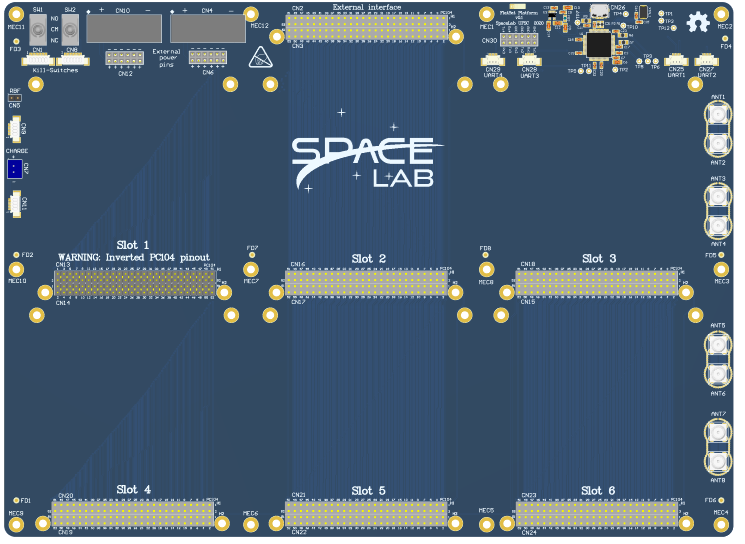
\includegraphics[width=0.8\textwidth]{figures/flatsat_top_image.png}
        \caption{FlatSat top PCB print.}
        \label{fig:pcb-top}
    \end{center}
\end{figure}

\begin{figure}[!ht]
    \begin{center}
        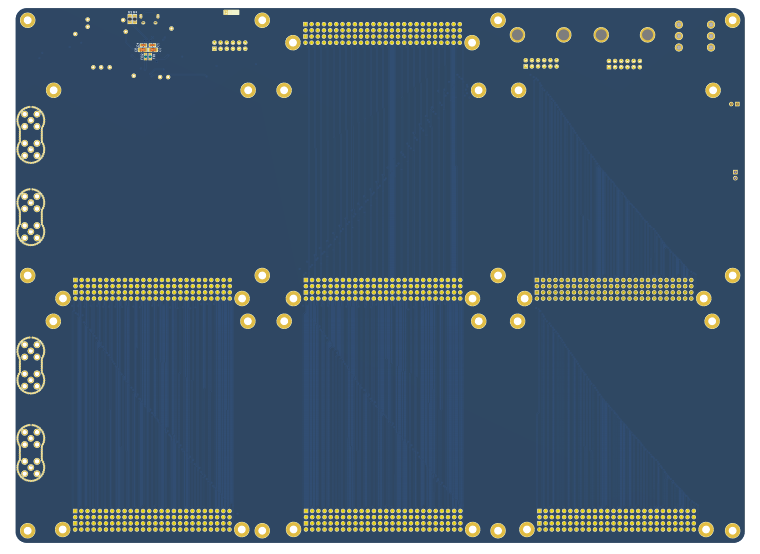
\includegraphics[width=0.8\textwidth]{figures/flatsat_bottom_image.png}
        \caption{FlatSat bottom PCB print.}
        \label{fig:pcb-bottom}
    \end{center}
\end{figure}

\section{PC-104 Interfaces}

On SpaceLab's FlatSat Platform the PC-104 interfaces are composed by two 52 pins with 2.54 mm (0.1 inch) pitch connectors. Slots N$^{\circ}$2 to N$^{\circ}$7 has two \textit{SSW-126-01-G-D} and the slot N$^{\circ}$1 uses two \textit{TSW-126-07-G-D} connectors with inverted pinout, see Figures \ref{fig:n2-n7-slots} and \ref{fig:n1-slot}. All pins are interconected to flexiblesize the positioning of the modules on the platform. All slots have grounded unlabeled mounting holes for the modules, the labeled MEC1 to MEC12 holes are for the FlatStats stability feet.

\begin{figure}[!ht]
    \begin{center}
        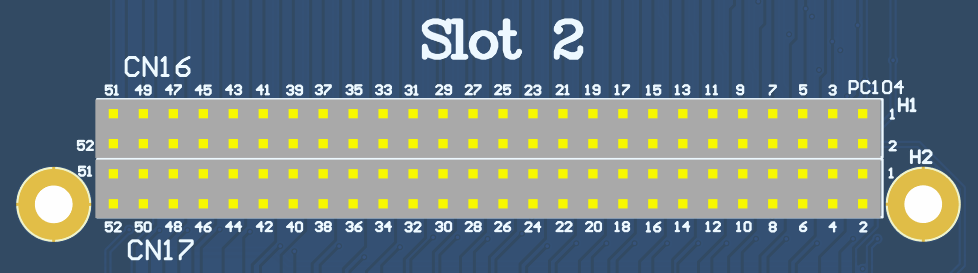
\includegraphics[width=0.75\textwidth]{figures/pc104_slots_n2_to_n7.png}
        \caption{FlatSat N$^{\circ}$2 PC-104 slot.}
        \label{fig:n2-n7-slots}
    \end{center}
\end{figure}

\begin{figure}[!ht]
    \begin{center}
        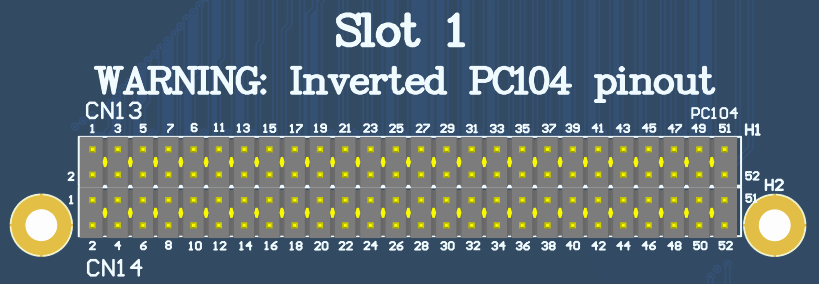
\includegraphics[width=0.75\textwidth]{figures/pc104_slot_n1.png}
        \caption{FlatSat N$^{\circ}$1 PC-104 slot.}
        \label{fig:n1-slot}
    \end{center}
\end{figure}

\section{Binding Posts and Power Receptacles}

Two sets of binding posts (\textit{4243-0}) can be mouted on the labeled CN4 and CN10 hole pads to be used for two external power supplies, see \autoref{fig:binding-posts}. The modules are powered via external jumper wires to the 12 position receptacle connectors (\textit{BCS-106-L-D-TE}) labeled CN6 and CN12. On the silkscreen the plus (+) signs are the positive power pins while the minus (-) signs are the GND pins.

\begin{figure}[!ht]
    \begin{center}
        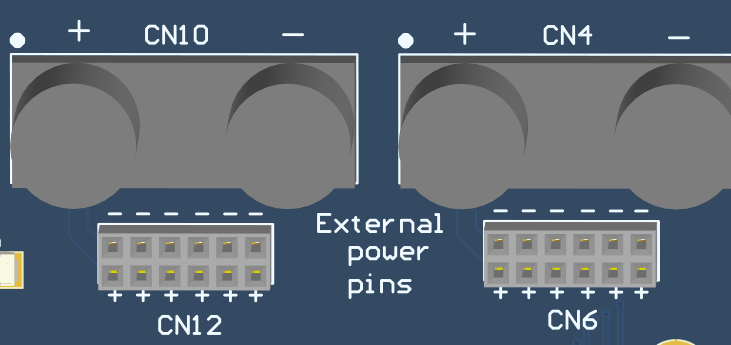
\includegraphics[width=0.75\textwidth]{figures/binding_posts.png}
        \caption{FlatSat binding posts and power receptables.}
        \label{fig:binding-posts}
    \end{center}
\end{figure}

\section{Charge Header}

On the board there is a JST XH 2 position header (\textit{B2B-XH-A-M(LF)(SN)}) for charging batteries, it can be seen in \autoref{fig:charge-connectors}. The component can suport up to 3000 mA of current, but it is advised to be used with less than 1500 mA. The 4 pin PicoBlade is to be connected to the EPS\nomenclature{\textbf{EPS}}{\textit{Electric Power System.}} module to make the interconnection for the JST header. The charge header also provides a detent lock for fastening and avoid a mistankenly reverse connection.

\begin{figure}[!ht]
    \begin{center}
        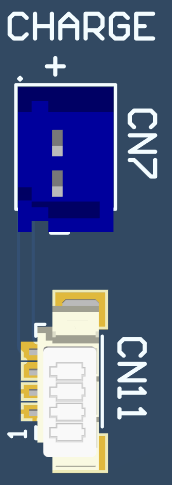
\includegraphics[width=0.15\textwidth]{figures/charge_connectors.png}
        \caption{FlatSat charge connectors.}
        \label{fig:charge-connectors}
    \end{center}
\end{figure}

\section{RBF Pin Header}

The platform has a RBF pin header that can seen \autoref{fig:rbf-connectors}. The interconnection between the header and the EPS module is done by a 4 pin PicoBlade.

\begin{figure}[!ht]
    \begin{center}
        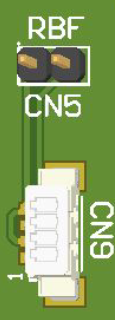
\includegraphics[width=0.15\textwidth]{figures/rbf_connectors.png}
        \caption{FlatSat RBF connectors.}
        \label{fig:rbf-connectors}
    \end{center}
\end{figure}

\section {SPDT Kill-Switches}

The kill-switches uses SPDT switches (\textit{100SP1T1B4M2QE}) for powering off the EPS module, see \autoref{fig:kill-switches-connectors}. The power off states are seen on \autoref{fig:kill-switches-states}, they are also present on the hardware schematics. The SPDTs are interconnected to the EPS module via two 6 pin PicoBlade connectors labeled CN1 and CN8.

\begin{figure}[!ht]
    \begin{center}
        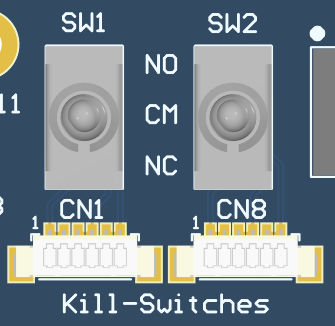
\includegraphics[width=0.5\textwidth]{figures/kill_switches_connectors.png}
        \caption{FlatSat kill-switches connectors.}
        \label{fig:kill-switches-connectors}
    \end{center}
\end{figure}

\begin{figure}[!ht]
    \begin{center}
        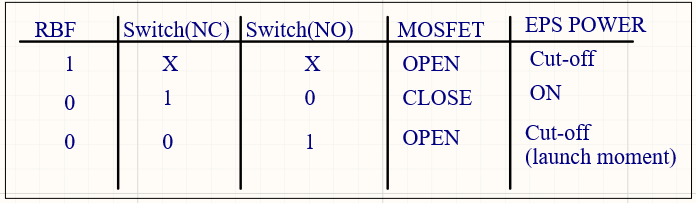
\includegraphics[width=0.75\textwidth]{figures/kill_switches_states.png}
        \caption{FlatSat kill-switches states.}
        \label{fig:kill-switches-states}
    \end{center}
\end{figure}

\section{Antenna Interfaces}

\subsection{SMA connectors}

On the PCB there are SMA connectors (\textit{132134-15}) labeled ANT1 to ANT8 for connecting VHF\nomenclature{\textbf{VHF}}{\textit{Very High Frequency.}}, UHF\nomenclature{\textbf{UHF}}{\textit{Ultra High Frequency.}} and S-Band antennas, see \autoref{fig:antennas-smas}. The receiver (RX) antenna is to be connected to one of the SMA, while the transmitter (TX) goes to the other connector and to the CubeSat module. The impedance control (see \autoref{fig:rf-track-width-calc}) and power dissipation (see \autoref{fig:rf-track-width-power-calc}) where approximately calculated for all 3 bands. As the FlatSat platform is to be used in light testing the aproximations where considered acceptable for the project.

\begin{figure}[!ht]
    \begin{center}
        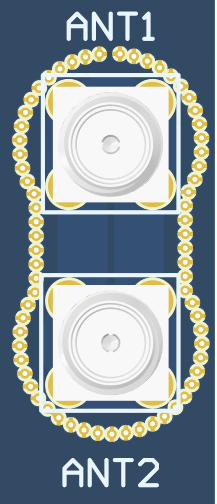
\includegraphics[width=0.15\textwidth]{figures/antennas_smas.png}
        \caption{FlatSat SMA connectors.}
        \label{fig:antennas-smas}
    \end{center}
\end{figure}

\subsection{Impedance Control of the RF Tracks}

\begin{figure}[!ht]
    \begin{center}
        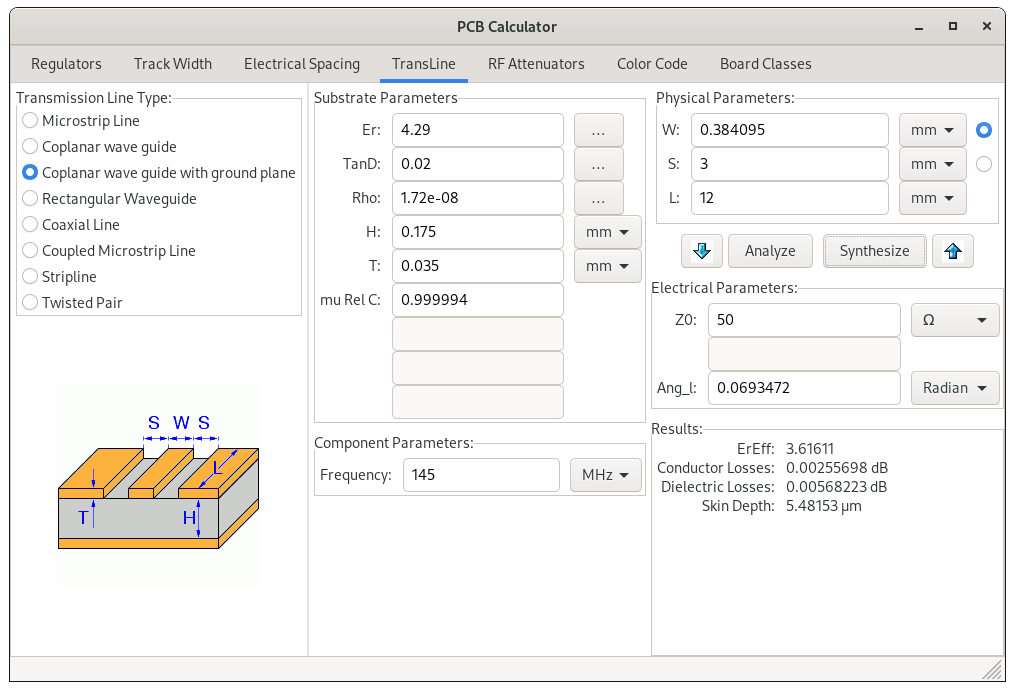
\includegraphics[width=\textwidth]{figures/rf-track-width.png}
        \caption{Calculation of the width of the RF tracks.}
        \label{fig:rf-track-width-calc}
    \end{center}
\end{figure}

\begin{figure}[!ht]
    \begin{center}
        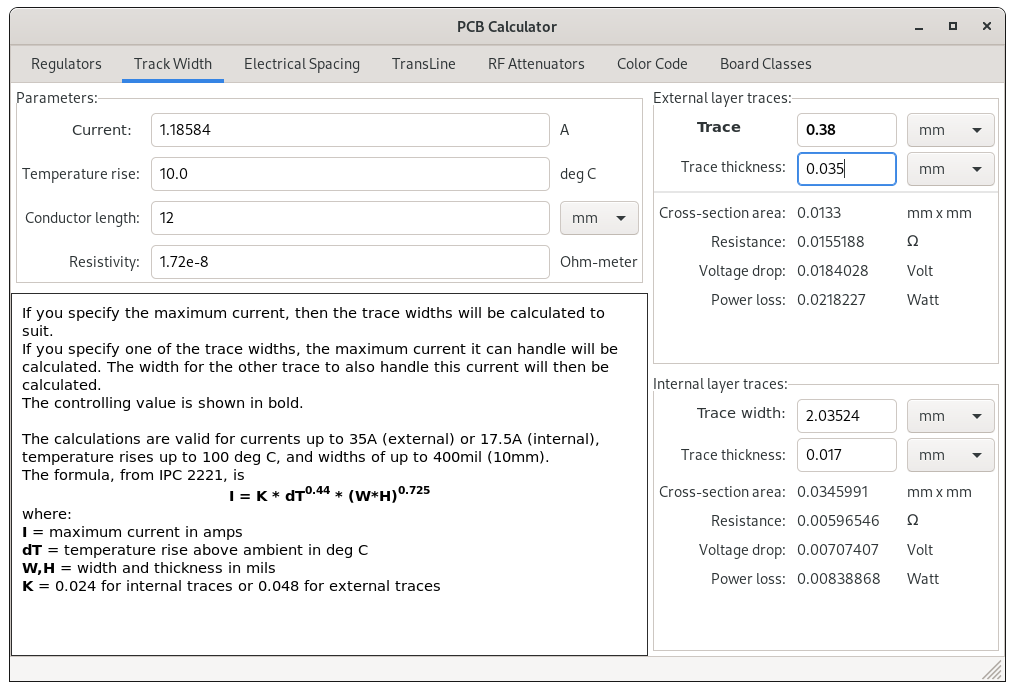
\includegraphics[width=\textwidth]{figures/rf-track-width-power.png}
        \caption{Power dissipation of the RF tracks.}
        \label{fig:rf-track-width-power-calc}
    \end{center}
\end{figure}

\section{UART to USB Converter}

There is a UART to USB converter circuit built-in the FlatSat platform for debbuging pourposes for four independent modules, it can be seen on \autoref{fig:ft4232h-circuit}. The subcircuit is self powered from a USB cable connecting a computer to a micro USB type B port (\textit{10118194-0001LF}). The USB Bridge converter IC\nomenclature{\textbf{IC}}{\textit{Integrated Circuit.}} is the \textit{FT4232HL-REEL} from FTDI. PicoBlade connectors are used for connecting the IC to the modules, see Figures \ref{fig:uart-picoblades-1} and \ref{fig:uart-picoblades-2}. It is also possible to use jumper wires connecting the 12 Position receptacle connector (\textit{BCS-106-L-D-TE}) labeled CN30 to the modules if PicoBlades are not used.

\begin{figure}[!ht]
    \begin{center}
        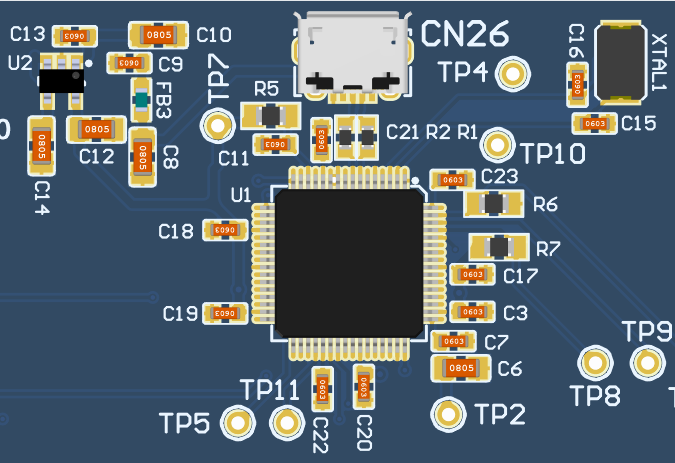
\includegraphics[width=0.75\textwidth]{figures/ft4232h_circuit.png}
        \caption{Top view of the UART to USB converter circuit.}
        \label{fig:ft4232h-circuit}
    \end{center}
\end{figure}

\begin{figure}[!ht]
    \begin{center}
        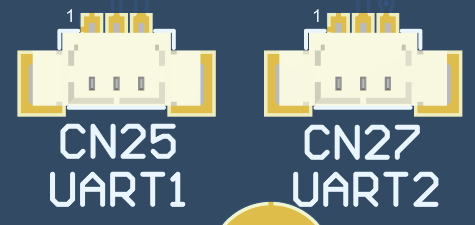
\includegraphics[width=0.5\textwidth]{figures/picoblade_uarts_n1_and_n2}
        \caption{UART PicoBlade N$^{\circ}$1 and N$^{\circ}$2 connectors.}
        \label{fig:uart-picoblades-1}
        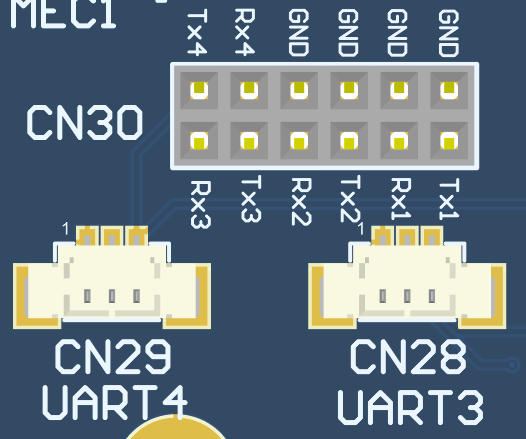
\includegraphics[width=0.5\textwidth]{figures/picoblade_uarts_n3_and_n4_and_receptable.png}
        \caption{UART PicoBlade N$^{\circ}$3 and N$^{\circ}$4 connectors and receptable.}
        \label{fig:uart-picoblades-2}
    \end{center}
\end{figure}

\section{Test Points}

The FlatSat has test points for the UART to USB converter circuit. The \autoref{tab:testpoints} displays their labels and description.

\begin{table}[!h]
    \centering
    \begin{tabular}{cllll}
        \toprule[1.5pt]
        \textit{Label} & \textit{Description} \\
        \midrule
        TP1                & (VPLL) 3V3 FT4232H power input. \\
        TP2                & (VREGOUT) 1V8 FT4232H internal power output. \\
        TP3                & (VPHY) 3V3 FT4232H power input. \\
        TP4                & (REF) Current reference for FT4232H. \\
        TP5                & (RESET\#) Reset input for FT4232H. \\
        TP6                & (EECS) EEPROM chip select - pulled down by 10k resistor. \\
        TP7                & (VCCIO) I/O interface 3V3 power supply input. \\
        TP8                & (EEDATA) EEPROM data I/O - pulled up by 10k resistor. \\
        TP9                & (EECLK) Clock signal to EEPROM - not used. \\
        TP10               & (PWREN\#) Active low power-enable output. \\
        TP11               & (SUSPEND\#) Active low when USB is in suspend mode. \\
        TP12               & (GND) 0V ground input for FT4232H.\\
        \bottomrule[1.5pt]
    \end{tabular}
    \caption{FlatSat test points.}
    \label{tab:testpoints}
\end{table}
